\documentclass[main.tex]{subfiles}

\begin{document}

\subsection{Primo esercizio}

\begin{figure}[H]
\centering
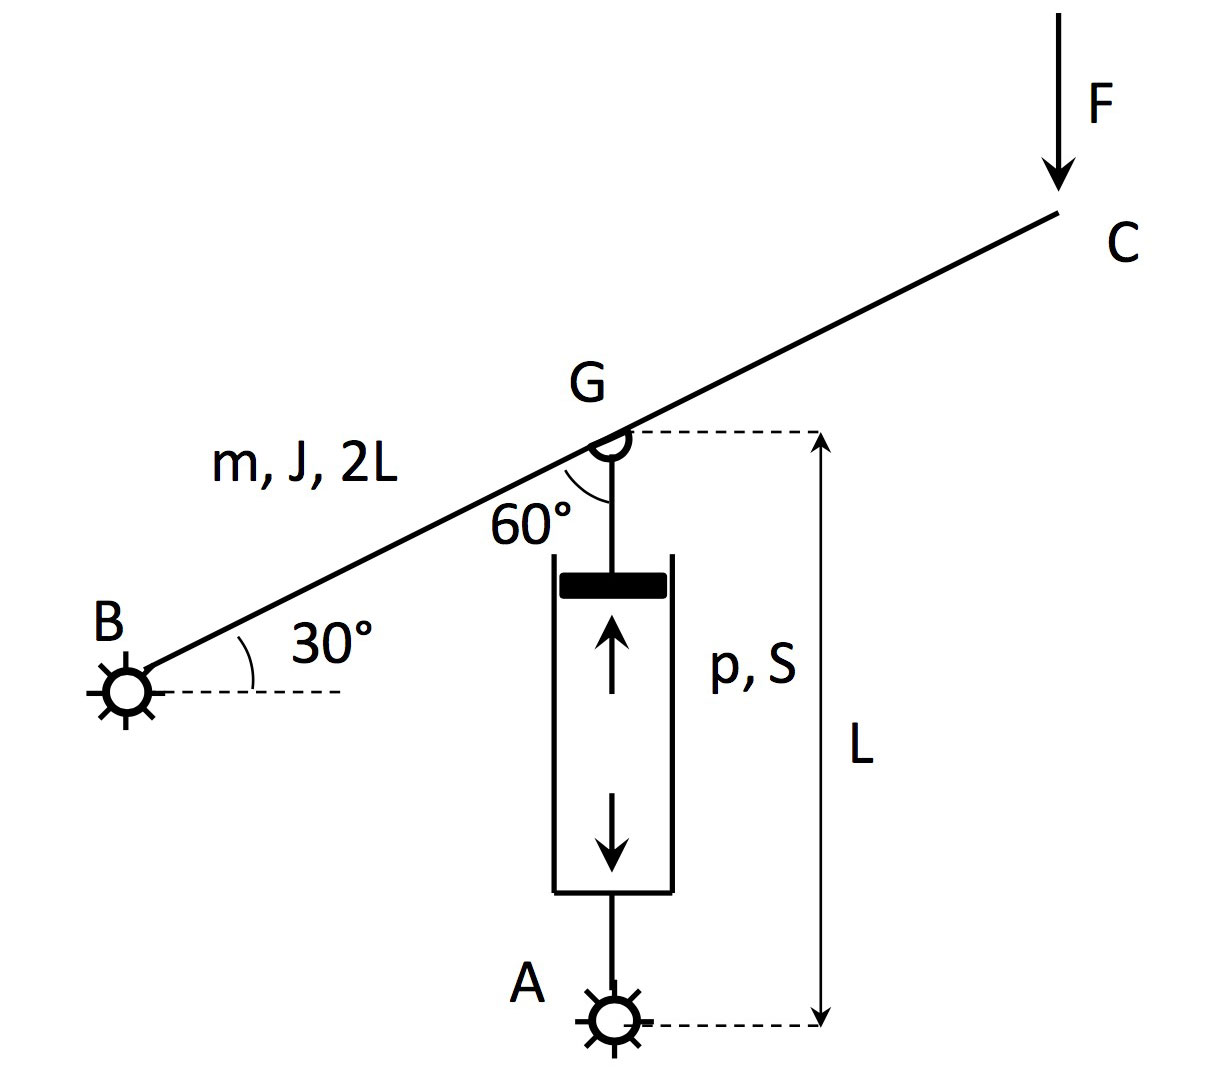
\includegraphics[width=0.75\textwidth]{2014-0407-1.jpg}
\end{figure}

\[
	L = 2\,m \quad
	S = 0.02\,m^2 \quad
	m = 200\,kg \quad
	J = 50\,kg m^2 \quad
	v = 0.2\,m/s \quad
	F = 5000\,N \quad
\]

Il sistema rappresentato in figura è posto nel piano verticale. L'asta BC è vincolata a terra con una cerniera in B e ha massa $m$, momento d'inerzia baricentrico $J$ e lunghezza $2L$. A tale asta, nel baricentro G (posto a metà dell'asta), è collegato un attuatore idraulico (di massa trascurabile), il cui estremo inferiore è incernierato a terra in A. Si consideri pari a S l'area del pistone e pari a p la pressione dell’olio nell'attuatore (si ricorda che le due forze uguali ed opposte esercitate dall’olio sul cilindro e sul pistone hanno modulo pari a $p*S$).
Nella posizione considerata, la lunghezza complessiva dell'attuatore è pari ad $L$. Sull'asta BC, nel punto C, agisce una forza $F$, diretta come in figura.

Nota la geometria del sistema e assegnate la forza F e la velocità $v$ di sfilo dell'attuatore (costante), si chiede di calcolare:
\begin{enumerate}
\item La velocità e l’accelerazione del punto C.
\item La pressione dell’olio all'interno dell'attuatore, necessaria per garantire la condizione di moto assegnata.
\end{enumerate}

\clearpage

\end{document}
